\documentclass[preprint]{elsarticle}
\biboptions{round, numbers}
\usepackage[latin1]{inputenc}
%\usepackage[T1]{fontenc}
%\usepackage{textcomp}
\usepackage{graphicx}
\usepackage{color}
%\usepackage{setspace}
\usepackage{url}
\usepackage[english]{babel}

\begin{document}

\begin{frontmatter}

%%%%%%%%%%%%%%%%%%%%%%%%%%%%%%%   TITLE   %%%%%%%%%%%%%%%%%%%%%%%%%%%%%%%

\title{A Review on Corporate Security Solutions. A Comparison with a User-Centric and Self-Adapted System}

%%%%%%%%%%%%%%%%%%%%%%%%%%%%%%%   AUTHORS   %%%%%%%%%%%%%%%%%%%%%%%%%%%%%%%

\author{P. de las Cuevas, A.M. Mora, J.J. Merelo}
\ead{\{paloma, amorag, jmerelo\}@geneura.ugr.es}
\address{Departamento de Arquitectura y Tecnolog�a de Computadores.\\ ETSIIT - CITIC. University of Granada, Spain}
%\author{A. M. Mora}
%\ead{amorag@geneura.ugr.es}
%\address{Departamento de Arquitectura y Tecnolog�a de Computadores. Escuela T�cnica Superior de Ingenier�as Inform�tica y de Telecomunicaci�n. CITIC. University of Granada, Spain}

%\maketitle

%
%%%%%%%%%%%%%%%%%%%%%%%%%%%%%%%%%   ABSTRACT   %%%%%%%%%%%%%%%%%%%%%%%%%%%%%%%%%
%
\begin{abstract} 
Enterprises, and their Chief Security Officers (CSOs) particularly, want to be sure that their security policies are complied. This goal turned hard to achieve since employees are able to use their own devices (laptops, smartphones, and tablets) at work, or at home but for work purposes. As this is part of the Bring Your Own Device (BYOD) philosophy and is being adopted by many companies everyday, a number of solutions have arisen in order to adapt it securely. In this paper, the most relevant solutions are presented, and so is displayed the European MUSES (Multiplatform Usable Endpoint Security) project, which tries to go further taking into account user behaviour for security rules adaption.
\end{abstract}

%
%%%%%%%%%%%%%%%%%%%%%%%%%%%%%%%%%   KEYWORDS   %%%%%%%%%%%%%%%%%%%%%%%%%%%%%%%%%
%
\begin{keyword}
BYOD \sep Corporate mobile security \sep End-to-end security solutions \sep User-centric systems \sep Self-adaptation \sep Multiplatform
\end{keyword}

\end{frontmatter}


%-------------------------------------------------------------------------------
%%%%%%%%%%%%%%%%%%%%%%%%%%%%%%%   INTRODUCTION   %%%%%%%%%%%%%%%%%%%%%%%%%%%%%%%
%-------------------------------------------------------------------------------

\section{Introduction}
\label{sec:intro}

Some years ago, company data were stored in own servers which were accessed by the employees or users by means of desktop or portable computers. Nowadays it is frequent that these data are distributed among multiple machines, even not all belonging to the company, and being consulted and modified through a wide amount of devices, some of them owned by the company's users. This is the so-called Bring Your Own Device (BYOD) philosophy. It is becoming highly successful due to the impact that smartphones and tablets are having in the market.
Data security and privacy are key factors for a company, thus, to protect them, it is usual to define Organisational Security Policies. Their definition is nowadays a very difficult problem, since the BYOD tendency means that several factors must be considered \cite{Opp_Security11}, most of them previously ignored or non-considered in the security systems, for instance the current mixture between personal and professional information in these devices (the user could navigate inside social networks where there could be friends and also company partners or clients).

Moreover, it has been demonstrated that people are the main hazard regarding the company security \cite{Adams_Users05}, so in this situation, some monitorization and security-aimed applications are arising, aiming to cope with the concept of seamless working experience on different devices. 
This concept is a methodology of work which allows users to start/continue a working session over multiple devices and locations without any significant loss of data. This new situation has a big impact from the point of view of the security \cite{Schu_SecPatterns05}, since the company's data borders have changed in the last years so now the users can access significant data from outside the enterprise, and possibly through a non absolutely secure channel.

In this scenario several solutions have arisen in order to manage the corporate security. Most of them try to be non-intrusive (regarding the users' personal data), friendly and easy to manage. This paper presents an overview of the main solutions, describing their features, and comparing them with a novel (still in development) system.

In addition, the paper introduces (giving an overview) a novel system, named MUSES, Multiplatform Usable Endpoint Security system. It is being implemented inside an European project and will provide a device independent, user-centric, and self-adaptive corporate security system, to deal with the aforementioned seamless working.
MUSES will analyse the users' behaviour and predict, using computational intelligence methods, risky or dangerous actions regarding both an event correlation and a risk and trust analysis engines. The system will be able to learn from the past user's behaviour, and react in a non-intrusive way to the potentially dangerous sequence of actions that he or she is conducting at any time.

The rest of the paper is organized as follows. First, some background situation about corporate secure networks is presented in Section \ref{sec:preliminaryconcepts}, explaining how BYOD affects to them. Then, some solutions from different companies are detailed in Section \ref{sec:toolsreview}, being specified for each one if the correspondent tool is available or, if not, the approximate release date. Some solutions are focused only in smartphones, while others are thought for laptops; also some are for a certain platform, but others remain multiplatform. 
Then, in Section \ref{sec:muses}, the Multiplatform End-Point Security System is presented. Its advantages and benefits in the comparison with the other solutions are commented in Section \ref{sec:comparison}.
Finally, the conclusions are discussed in Section \ref{sec:conclusions}.


%----------------------------------------------------------------------------
%%%%%%%%%%%%%%%%%%%%%%%%%%%%%%%   BACKGROUND  %%%%%%%%%%%%%%%%%%%%%%%%%%%%%%%
%----------------------------------------------------------------------------


\section{Preliminary concepts and background about enterprise security}
\label{sec:preliminaryconcepts}

Until these days, enterprises used to follow a static policy devoted to controlling a certain structure\cite{BYOD13}, where the assets and the devices were purchased and maintained by the company. Now that corporate networks are becoming dynamic for being adapted to the BYOD philosophy, there is an additional risk because the devices that the employees use are not always company-owned.

On the other hand, employee-owned devices like smartphones, they are not just for work purposes anymore. As the name says, smartphones are more than simple old cell phones, and people who use them in their works have the possibility of having a good balance between work and private life. For this reason, the risk of uncontrolled devices accessing to corporate access in unsafe conditions, due to the number of risky applications, is bigger.

Then, it is necessary to take into account the security in an outsourced enterprise model. Figure \ref{fig:outsourced_sol_img} presents an example situation in which some of the mobile services have been outsourced to an external operator, typically a telecommunications operator.
The functional elements are the same ones as in an enterprise managed solution. For instance, the demilitarized zone, the intranet wired and WiFi zones, the Intrusion Detection System (IDS)\cite{ids13}, or the mail and VPN servers. However some of them have been moved outside the enterprise. Of course the moved elements try to exemplify the most typical outsourced components for enterprises having a mobile device strategy.
The main differences are related to the possible outsourcing of the:

\begin{enumerate}
	\item \textbf{Network Access Control (NAC):} it checks that mobile devices satisfy a set of prerequisites (e.g., OS patch level, antivirus properties, etc.) before allowing them connecting to the intranet. Normally it manages the accesses to the Intranet WiFi net, but it can also be involved in controlling Virtual Private Network (VPN) accesses.
	\item \textbf{Active Directory Domain Controller (ADDC):} this service exemplifies the network management framework in charge of authenticating devices and users, as well as of distributing enterprise security policies.
	\item \textbf{MDM Server:} many telecommunications operators are deploying Machine-to-Machine (M2M)\cite{m2m12} management frameworks, and start offering related services that, among other features, provide features for managing mobile devices. The telecommunications operators can play a relevant role especially in BYOD scenarios due to their habits of subscription plans including medium-to-high end smart phones or tablets;
	\item \textbf{Applications Store:} there is a big interest of telecommunications operators for the so called \textit{mobile ecosystem}, i.e. services tied to mobile devices and to mobile device apps. One of the key elements of this mobile ecosystem is the controlled provisioning of apps or content targeted to meet enterprise requirements, especially Small and Medium Enterprises (SME). In Figure \ref{fig:outsourced_sol_img} the telecommunications operator manages a Private/Hybrid App Store to exemplify both situations in which the operated App Store provides and manages exclusively enterprise specific apps (Private Application Store), as well as enterprise and operator or third parties apps (Hybrid App Store).
	\item \textbf{Mail Server:} enterprises having a consistent base of employees or collaborators using mobile devices often prefer the outsourcing of the enterprise mail service (or use fully outsourced \textit{Productivity Suites}\cite{suites12}) to reduce costs, configuration and management issues, and improve service quality.
\end{enumerate}

\begin{figure}
	\begin{center}
		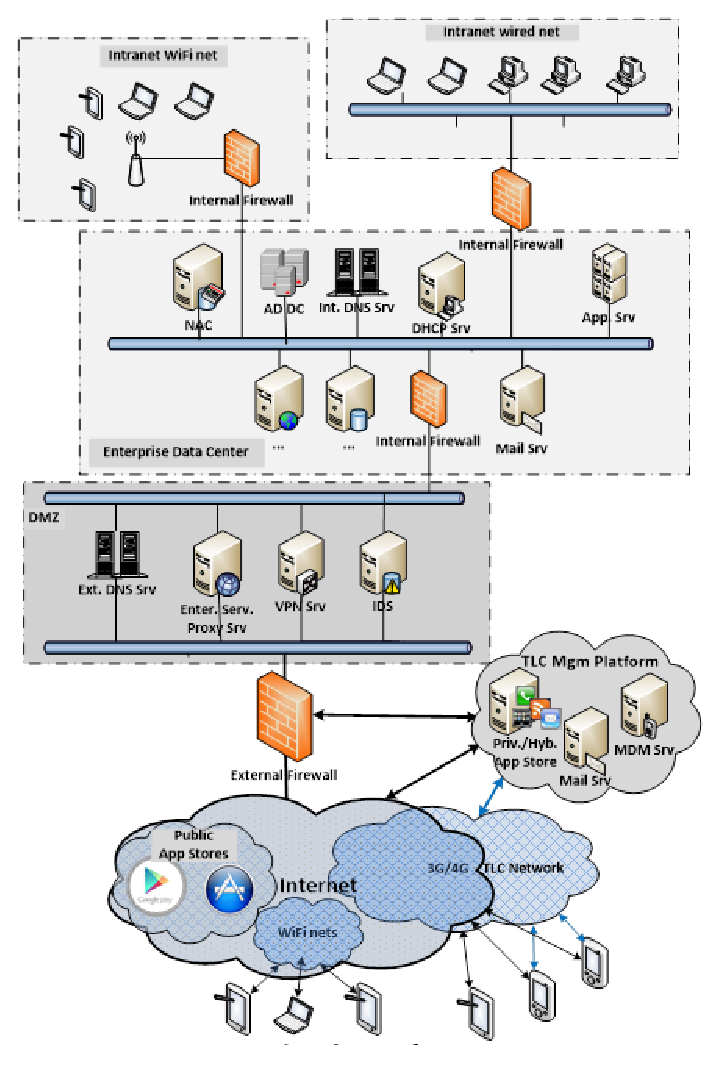
\includegraphics[scale=0.7]{img/outsourced_solution.eps}
		\caption{Security architecture model of an enterprise in which some of the mobile services have been outsourced to an external operator.}
	\label{fig:outsourced_sol_img}
	\end{center}
\end{figure}

%------------------------------------------------------------------------------
%%%%%%%%%%%%%%%%%%%%%%%%%%%%%%%   TOOLS REVIEW  %%%%%%%%%%%%%%%%%%%%%%%%%%%%%%%
%------------------------------------------------------------------------------

\section{Tools for corporate mobile security}
\label{sec:toolsreview}

Now that BYOD philosophy is a trend, a number of tools have been designed specifically for CSOs and Chief Information Security Officers (CISOs) to secure, monitor, and control spartphones and other personal mobile or portable devices. Some of these tools have influenced the development of the European MUSES project itself, showed in \ref{sec:muses}. This section presents the products that can be considered related to MUSES objectives.

% Don't completely like the intro for being too focused to MUSES.

%----------------------------------------------------------------------------

\subsection{IBM Hosted Mobile Device Security Management}
\label{subsec:ibm}

One of the first companies who supported the BYOD model was IBM in 2011, as they recognized the increase of employees who brang their personal smartphones or tablets into the workplace. To help organizations\cite{ibm11} embrace both company and employee owned mobile devices (as said, this practise is part of the BYOD model) in a security-rich environment, IBM developed a mobile device security management solution. For IBM, a mobile security strategy should focus on several key areas.

On one hand, the organization should identify which business data the strategy will allow to be stored and processed on which mobile devices. This helps determine what needs to be protected and to what degree. Then, because different mobile platforms have different native security mechanisms, the organization needs to define which mobile device platforms will be allowed in the business environment and, thus, need to be supported in the mobile security strategy and plan. Also there is need to decide the responsibility for mobile security management work, whether using the current IT security team to handle mobile devices, or outsourcing to a managed security service provider. And no matter what the mobile environment, a number of mobile security policies and best-practise procedures need to be put in place and should also be identified in the company's mobile security strategic plan.

Taking into account these considerations, IBM developed a framework that specifies security domains and levels for applying various security technologies. When applied to mobile devices, the framework suggests the following security controls, with actual requirements varying by deployment. The features of this framework are detailed in Table \ref{tab:IBMframework}.

\begin{table}
	\caption{IBM Hosted Mobile Device Security Management framework}
	\label{tab:IBMframework}
	\begin{tabular}{ p{11cm} }
		\hline
		\textbf{Identity and access}\\
		\hline
		Enforce strong passwords to access the device.\\
		Use site authentication or two-factor user authentication to help increase the trustworthiness between a user and a website.\\
		If VPN access to corporate intranet is allowed, include capability to control what IP addresses can be accessed and when re-authentication is required for accessing critical resources.\\
		\hline
		\textbf{Data protection}\\
		\hline
		Encrypt business data stored on the device and during transmission.\\
		Include capability to wipe data locally and remotely.\\
		Set timeout to lock the device when it is not used.\\
		Periodically back up data on the device so data restore is possible after the lost device has been recovered.\\
		Include capability to locate or lockout the device remotely.\\
		\hline
		\textbf{Application security}\\
		\hline
		Download business applications from controlled locations.\\
		Run certified business applications only.\\
		Monitor installed applications and remove those identified to be untrustworthy or malicious.\\
		\hline
		\textbf{Fundamental integrity control}\\
		\hline
		Run antimalware software to detect malware on storage and in memory.\\
		Run a personal firewall to filter inbound and outbound traffic.\\
		Integrate with the company's VPN gateway so a device's security posture becomes a dependency for intranet access.\\
		\hline
		\textbf{Governance and compliance}\\
		\hline
		Incorporate mobile security into the company's overall risk management program.\\
		Run a personal firewall to filter inbound and outbound traffic.\\
		Include mobile devices in the company's periodic security audit.\\
		\hline
	\end{tabular}
\end{table}

Regarding IBM hosted mobile device security solution's architecture, the solution is built on a sound client-server architecture in which the server centrally controls and manages security policies and settings for various security features. The client would be installed on the mobile device and regularly communicate with the server to enforce policies, execute commands and report status. Also, IBM's solution contains reporting and analysis capabilities, with information that helps the company to support policy and regulation compliance, recognize the mobile threat landscape and evaluate the solution's effectiveness in countering threats.

%----------------------------------------------------------------------------

\subsection{Sophos Mobile Control}
\label{subsec:sophos}

Sophos is a company founded in 1985 focused on IT security and data protection for businesses. Their ``Mobile Device Management'' main product is Sophos Mobile Control. It is oriented to IT administration for mobile devices, trying to offer to the users the possibility of choosing the delivery model to suit their needs, i.e., between on-premise and Software as a Service (SaaS).

The tool offers the possibility of managing all workers and co-workers smartphones and tablets from a single-based console. The console monitors the devices throughout their full lifecycle: from the initial set up and enrolment, right through to decommissioning. Other features are similar to IBM's product, adding some new like being able to connect to an existing user directory using Lightweight Directory Access Control (LDAP)\footnote{LDAP is an application protocol for accessing and maintaining distributed directory information services over an Internet Protocol (IP) network.}.
	
Additional security is provided by the incorporation of Malware and Web protection. Regarding compliance Enforcement, the main goal is not to sacrifice company's security in favour of flexibility for the users. Company's BYOD initiative should include an Acceptable Use Policy to ensure the users are aware of any measures the company may take if a device breaches the security policies. This is reachable by doing three main tasks. First, by enforcing Security Policies, that means allowing setting up user and group-based security policies. The security settings can also vary from one platform to another, thus is necessary to set task bundles and individual actions for many different violations. Secondly, risk mitigation: these actions can be set according to the severity of a breach. For minor cases, the company may want to simply inform the user. If sensitive data is at risk, a remote wipe may be the only viable option. The actions vary for each platform, but the most common platforms such as Android and iOS allow blocking email access, notifying the admin, performing a remote lock or wiping, locating a device using 3D maps, triggering a remote alarm, transferring a task bundle combining a number of actions, and Sophos Mobile Security adds the possibility of trigger a scan. Finally, compliance check, i.e. the settings available in the compliance check vary for each platform. Some of the most widely used features include allow or disallow root rights or jailbreaking, allow/disallow app downloads from non-market app stores, require encryption, and whitelist or blacklist apps. Additionally, Sophos Mobile Security allows disallowing malware apps, set maximum intervals since last Mobile Security scan, and allow or disallow suspicious apps and potentially unwanted apps (named PUAs).
	
Then, the Enterprise App Store in Sophos Mobile Control allows the company to supply the users with recommended and required apps directly on their device. Both company's in-house and app store apps are shown on the user's mobile device, where they can click to trigger the installation. Also, one of company's goals is to keep the employees working without increasing the burden for the IT department. The self-service portal built-in included in Sophos Mobile Control has the following features:
	
	\begin{enumerate}
		\item Allow users to register their own devices and agree to an acceptable use policy that the company has defined.
		\item Let them use their personal device as part of the BYOD program, and the company can make sure it is secured.
		\item The users can choose to remotely locate, lock or wipe their devices and reset their passcode without having to contact the company help desk.
		\item Provide a step-by-step process when they register a device. All profiles, including email access, are available after registration.
		\item The company define which features are available in its self-service portal from the administrator console.
		\item The users can access the portal from their mobile device or from any PC with Internet access.
	\end{enumerate}

%----------------------------------------------------------------------------

\subsection{Samsung's Knox Mobile Security Suite}
\label{subsec:samsungknox}

As part of its SAFE (Samsung for enterprise) brand, Samsung revealed at the Barcelona Mobile World Congress 2013 the Knox application, which will be available on his next Galaxy smartphone generation.
The main feature of this security package is the use of different containers for the business and the personal side. Each one even has its own set of wallpapers, in order to be more evident for the user. Figure \ref{fig:img_knox_01} shows the architecture followed by the application.
To enter the business side, it will be necessary to introduce a password. Nevertheless, no passwords will be required for the business applications anymore. The applications approved by the company IT department must meet Samsung's security standards and allow single sign-on. There will be over 338 IT policies that can be access via the Knox API. Also, Knox allows different VPNs for individual apps.
Regarding the information protection methods, data files saved by applications of each environment are encrypted with AES 256-bit algorithm, in such manner the container and only the container can access these files. In the same way, the user won't be able to share data between the two environments, i.e. there will be separate contact lists and the user cannot send a contact from one side to the other. Also, if the user copies data to the clipboard in the Knox container, it won't be there in the personal container. Other features of this tool are the following:

\begin{enumerate}
	\item Customizable Secure Boot - This ensures that only verified and authorized software can run on the device. It is a primary component that forms the first line of defence against malicious attacks on devices with Samsung KNOX. In addition, Samsung Knox's Secure Boot technology allows the switch of the secure boot root certificate in a secure manner after the devices are shipped.
	\item TrustZone-based Integrity Measurement Architecture (TIMA) - This runs in the secure-world and provides continuous integrity monitoring of the Linux kernel. When TIMA detects that the integrity of the kernel or the boot loader is violated, it takes a policy-driven action in response. One of these policy actions disables the kernel and powers down the device.
	\item Security Enhancements for Android - This feature provides an enhanced mechanism to enforce the separation of information based on confidentiality and integrity requirements. It isolates applications and data into different domains so that threats of tampering and bypassing of application security mechanisms are reduced while the amount of damage that can be caused by malicious or flawed applications is minimized.
\end{enumerate}

\begin{figure}
	\begin{center}
		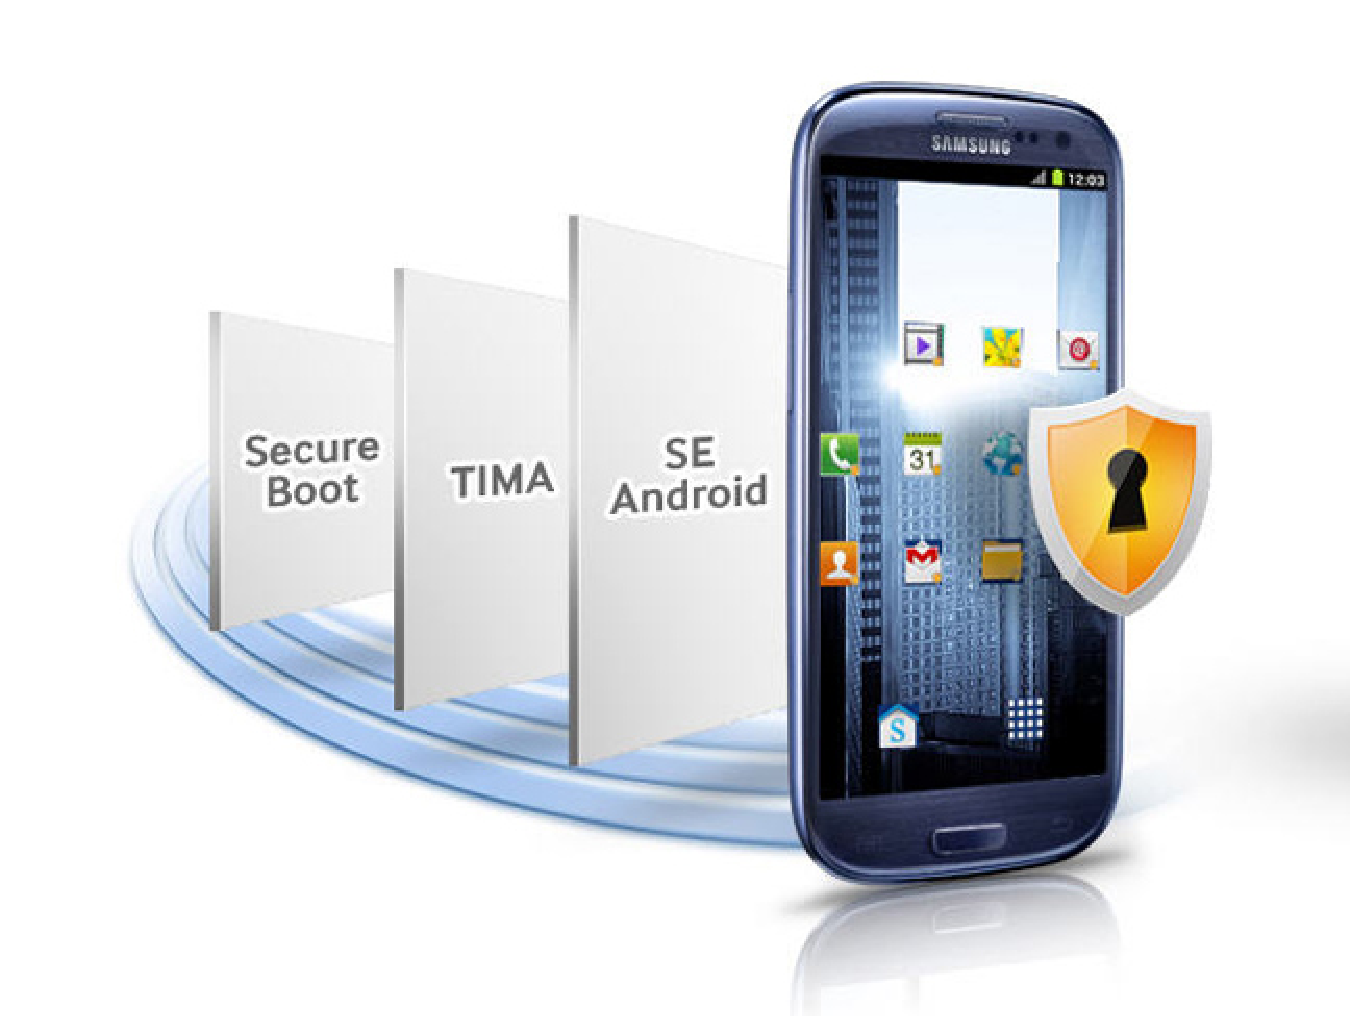
\includegraphics[scale=0.3]{img/samsung_knox_nueva.eps}
		\caption{Samsung's Knox utility architecture. Source: http://www.samsung.com/global/business/mobile/solution/security/samsung-knox}
	\label{fig:img_knox_01}
	\end{center}
\end{figure}

%----------------------------------------------------------------------------

\subsection{Good's Bring Your Own Device solution}
\label{subsec:goodsbyod}

Good Technology is a company that was founded in 1996 in California. The philosophy followed by Good is similar to Samsung's Knox one: to create a secure container that places an unreachable partition between personal and business data to protect email and other programs. The solutions that they offer are similar than the previous ones. They have focused in mobile (not laptops) devices, though they support a number of OSs, and in separarting personal and company data. A Good's secure Network Operations Center (NOC) is introduced for dealing with the unauthorised devices, or providing access to secure collaboration solutions (email, PIM, calendar), intranet, and in-house or third-party mobile applications. Finally, Good offers best practice recommendations to help the company's BYOD policies such as reimbursements and stipends. There is a document available at Good's webpage\footnote{\url{http://www1.good.com/mobility-management-solutions/bring-your-own-device}} which contains a number of questions about security policies and how to cope them all.

%----------------------------------------------------------------------------

\subsection{BlackBerry Balance}
\label{subsec:blackberrybalance}

This security package was announced as a feature of BlackBerry 10. Nevertheless, it is available with BlackBerry Enterprise Service 10, which is a device management, security and app management for BlackBerry, iOS and Android devices. When BlackBerry Balance is activated, these characteristics are available:

\begin{enumerate}
	\item Work data cannot be copied and pasted into personal apps. The device will display messages like the shown in Figure \ref{fig:blackberry_bal}.
	\item If a user attempts an action that is not permitted by IT policy or that may cause secure work information to come into contact with personal applications, the action won't be permitted.
	\item Employees can access the personal information and apps that keep them in touch with the people and things they care about, while staying connected to important work information when they need to perform.
	\item If the device gets lost or stolen, or if the employee leaves the organization, there will be an option to wipe just work information and it can be done remotely.
\end{enumerate}


\begin{figure}
	\centering
		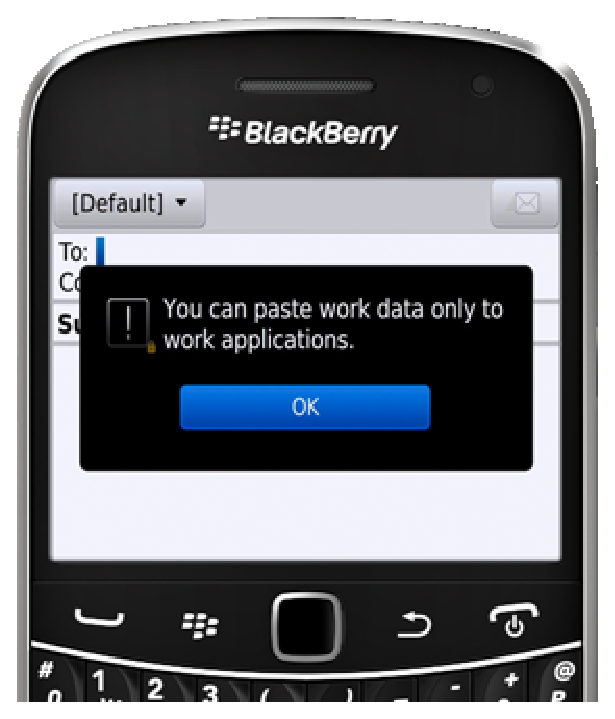
\includegraphics[scale=0.5]{img/Blackberry_balance.eps}
		\caption{Displayed message in new Blackberry 10 when attepmting to copy sensitive company data. Source: http://uk.blackberry.com/business/software/blackberry-balance.html.}
	\label{fig:blackberry_bal}
\end{figure}


%----------------------------------------------------------------------------
%%%%%%%%%%%%%%%%%%%%%%%%%%%%%%%%   MUSES %%%%%%%%%%%%%%%%%%%%%%%%%%%%%%%%%%%%
%----------------------------------------------------------------------------


\section{Multiplatform Usable Endpoint Security System}
\label{sec:muses}

MUSES system will work as presented in Figure \ref{fig:system_overview}. The user interacts with the devices, own or corporate, through the MUSES graphical interface and inside his or her own context (situation, connection, status). This application includes two modules, a \textit{controller} and an \textit{actuator}. The first one monitorizes the environment (context) and the user's behaviour, translating his/her actions into a sequence of events. These events, along with the patterns defining the user's conduct, are processed by the system in real-time by means of a Risk and Trust Analysis Engine (RT2AE) and an Event Correlation module. Then, a decision is taken in the corporate security operations centre (SOC) side, considering the RT2AE output and the set of security rules adapted to that specific user and context. The correspondent feedback is communicated to the user through the \textit{actuator}, which is also in charge of triggering the recommended actions to stop the user's or application's doings, in case it is required.

\begin{figure}
\centering
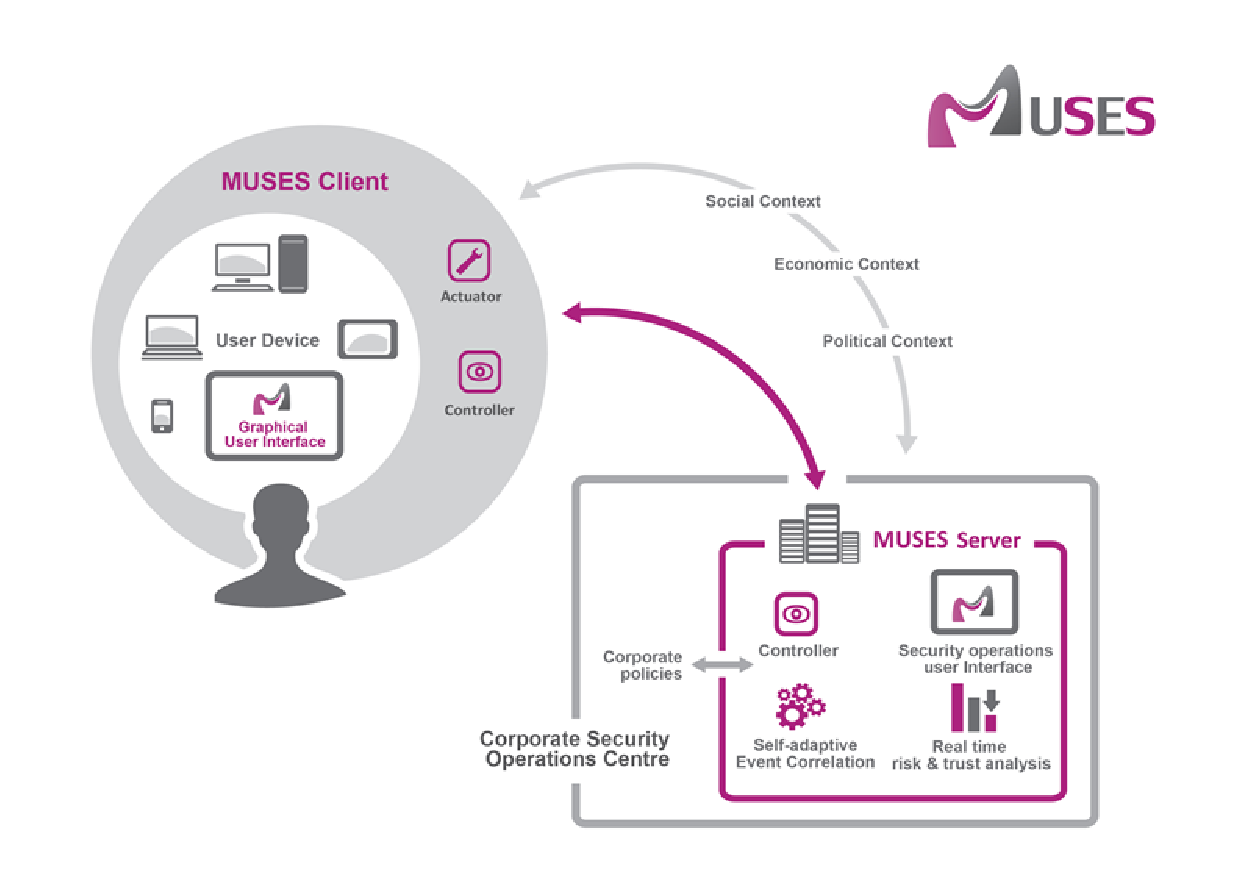
\includegraphics[scale=0.55]{img/system_overview.eps}
\caption{MUSES system overview.\label{fig:system_overview}}
\end{figure}

The system architecture can be seen in Figure \ref{fig:architecture}. It is a client-server approach in which the \textit{client} program will be installed in every user's device independently of the platform (operative system and type of device). This client contains a \textit{monitorization module}, which gathers the performed sequence of events and user context information; a \textit{controller module} in charge of take some light decisions considering the server response to the current situation (it will also take the control in case the device cannot connect with the server). The device controller will trigger the \textit{actuator} if necessary. This module will provide the user with some feedback, and will interact with the applications being monitorized if recommended or required.

The \textit{server} side would be installed in the corporate SOC. This application contains, in addition to an user interface to manage it, the main modules in the security-aimed decision process: the \textit{RT2AE} and the \textit{Event Correlator}. These components are connected between them and also with the main \textit{Controller}, that will connect with the device side sending the selected set of security rules that better fit with the current situation, along with the actions to be performed according to them.

\begin{figure}
\centering
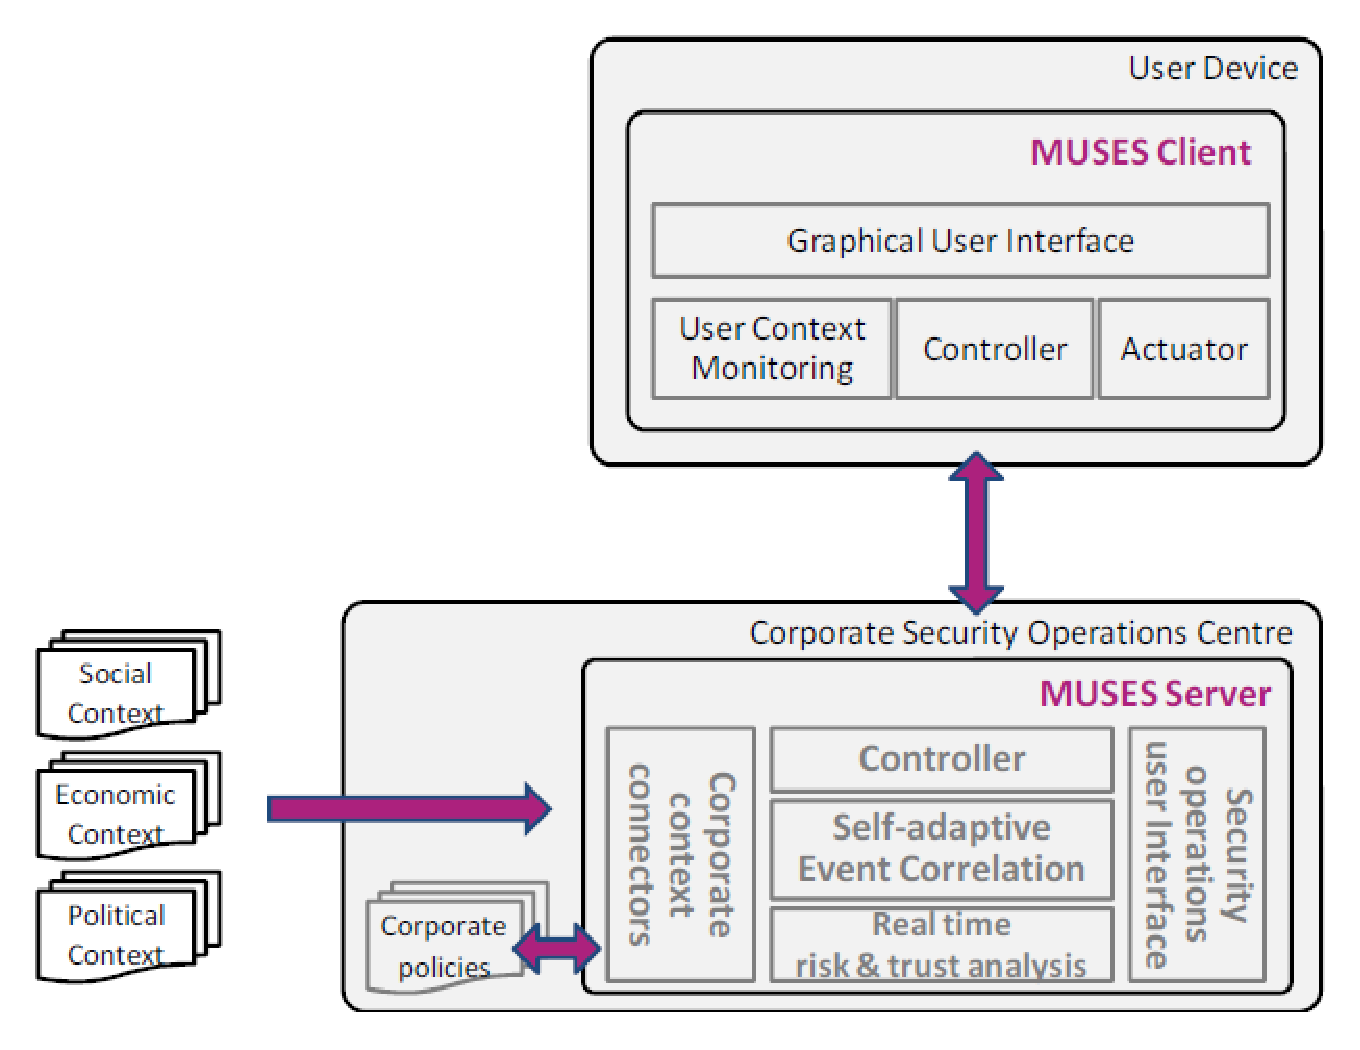
\includegraphics[scale=0.45]{img/architecture.eps}
\caption{Proposed architecture\label{fig:architecture}}
\end{figure}

One of the main features of the presented system is the self-adaptation (to the user and context) of the set of rules. To this aim, asynchronously to the system working, there will be run a process which will consider the whole amount of historic information regarding user's behaviour and context, and refine it by means of computational intelligence and machine learning techniques. Thus the set of security rules will be adapted to the every user in the system, updating some of the existent rules and creating new ones (always respecting the corporate security policies).
Moreover, some predictive models will be also obtained applying other soft computing techniques, so the user's potentially dangerous behaviour will be anticipated.


%MUSES (or Multiplatform Usable Endpoint Security) is a project co-funded by the European Commission under the Seventh Framework Programme. This MUSES project has concluded it first year (from a total of three) and is expected to develop a prototype (Prototype \#1) for Android Devices in the second year.
%The final product of MUSES for companies will be a system which will be installed in workers' devices and enterprise servers. There will be compiled versions of MUSES deployed on these kinds of devices:
%
%\begin{enumerate}
%	\item Portable devices. These are laptops that can be used in the company's premises or elsewhere.
%	\item Mobile devices. These include smartphones and tablets.
%	\item Enterprise servers.
%\end{enumerate}
%	
%The first two kinds can be owned either by the company itself or their employees (or their co-workers, where co-workers are indirect employees of the company; the term generally refers to the employees of contractor companies.).
%The very definition of MUSES as multiplatform usable endpoint security implies that the MUSES solution should be deployable and run on a number of platforms and operating systems. Being multiplatform is a key requirement for the adoption of MUSES as part of a wide range of corporate security strategies.
%
%In order to achieve its stated goals the MUSES system should be able to: capture user's behaviour, decide in real-time if user's behaviour poses a security threat, propose adaptations of the security policies based on patterns of user's behaviour, provide usable feedback to the user (based on security threat), and apply necessary adaptations and manipulation of context.

%----------------------------------------------------------------------------
%%%%%%%%%%%%%%%%%%%%%%%%%%%%%%%   COMPARISON  %%%%%%%%%%%%%%%%%%%%%%%%%%%%%%%
%----------------------------------------------------------------------------

\section{MUSES Advantages Against other Solutions}
\label{sec:comparison}


The main differences with MUSES, is that it will be also a free, open-source, platform independent solution. This is an important advantage because all the existent tools take into account only smartphones and tablets, but MUSES covers laptops and company PCs too. Moreover the companies need specific operative system and server (like Windows Server, for instance). Other big plus of the MUSES system is its new feature of self-adaptiveness. MUSES is able to adapt to changes, either regarding corporate security policies, newly discovered vulnerabilities or threats, different environments of use or user profiles. 

In addition, the existing products are mostly policy-based, but MUSES takes its decisions not only considering policies, but also based on the terminals/users context (location, connected networks and so on), to really understand the real danger of a specific action.


%----------------------------------------------------------------------------
%%%%%%%%%%%%%%%%%%%%%%%%%%%%%%%   CONCLUSIONS  %%%%%%%%%%%%%%%%%%%%%%%%%%%%%%%
%----------------------------------------------------------------------------

\section{Conclusions}
\label{sec:conclusions}

In this work, there were presented many tools that prove how information security in the enterprise is adapting to this emergent philosophy of BYOD. For each one, the main features and working environments were detailed. Also it was shown, by the introduction to MUSES project, how the European Community is specially aware about that and is developing a free solution for managing employees privacy, and securing companies' assets in this changing environment.

%%%%%%%%%%%%%%%%%%%%%%%%%%%%%  ACKNOWLEDGEMENTS %%%%%%%%%%%%%%%%%%%%%%%%%%%%%%%%

\section{Acknowledgements}
This work has been supported by MUSES FP7 project, and in part by the P08-TIC-03903 project awarded by the Andalusian Regional Government, the FPU Grant 2009-2942, and the TIN2011-28627-C04-02 project, awarded by the Spanish Ministry of Science and Innovation.

\bibliographystyle{elsarticle-num}

% Antonio - Poner la bibliograf�a en fichero .bib

\begin{thebibliography}{00}

\bibitem{ids13}
Theodor Sommestad, Admund Hunstad. \emph{Intrusion detection and the role of the system administrator.}, from Swedish Defence Research Agency (FOI), Link�ping, Sweden, 2013.

\bibitem{m2m12}
NTT DOCOMO, \emph{DOCOMO to Launch Global M2M Platform}, in M2M Magazine, December 2012.
http://www.machinetomachinemagazine.com/2012/12/05/docomo-to-launch-global-m2m-platform/.

\bibitem{suites12}
The Radicati Group Inc., report \emph{Microsoft Office 365 - Analysis and Forecast, 2012-2016}. June 2012. 

\bibitem{BYOD13}
Sandy Bacik, \emph{Security Implications of Bring Your Own Device, IT Consumerization, and Managing User Choices}, in Information Security Management Handbook, Sixth Edition, Volume 7, pp. 133--142, 2013.

\bibitem{ibm11}
I-Lung Kao, \emph{IBM Security Services. Securing mobile devices in the business environment}, IBM, 2011.

\bibitem{Adams_Users05}
A.~Adams and A.~Sasse.
\newblock {\em Users are not the enemy}.
\newblock Security and Usability: Designing Systems That People Can Use.
  O\'Reilly Associations, 2005.

\bibitem{Blackberry_tool}
Blackberry.
\newblock Blackberry balance.
\newblock http://es.blackberry.com/business/software/blackberry-balance.html.

\bibitem{IBM_tool}
IBM.
\newblock Hosted mobile device security management.
\newblock
  http://www-935.ibm.com/services/us/en/it-services/managed-security-services-cloud-computing-hosted-mobile-device-security-management.html.

\bibitem{Opp_Security11}
R.~Oppliger.
\newblock Security and privacy in an online world.
\newblock {\em IEEE Computer}, 44(9):21--22, September 2011.

\bibitem{Samsung_tool}
Samsung.
\newblock Knox.
\newblock
  http://www.samsung.com/global/business/mobile/solution/security/samsung-knox.

\bibitem{Schu_SecPatterns05}
M.~Schumacher, E.~Fernandez-Buglioni, D.~Hybertson, F.~Buschmann, and
  P.~Sommerlad.
\newblock {\em Security Patterns: Integrating Security and Systems
  Engineering}.
\newblock John Wiley \& sons, 2005.

\bibitem{Sophos_tool}
Sophos.
\newblock Mobile control.
\newblock http://www.sophos.com/en-us/products/mobile-control.aspx.

\bibitem{Good_tool}
G.~Technology.
\newblock Byod solution.
\newblock
  http://www1.good.com/secure-mobility-solution/bring-your-own-device.html.


%Para fijarme
%\bibitem{GAs_Goldberg89}
%Goldberg D.E., Korb B., Deb K., \emph{Messy genetic algorithms: motivation, analysis, and first results}, Complex Systems, 3(5), pp. 493--530, 1989.


\end{thebibliography}

\end{document}
